% =====================================================================
% ACM Research Summer Internship 2026 — Internship Report
% Project: DTSG (Dynamic Temporal State Graph)
%
% Placeholders to fill before submission are marked  % <<< FILL
% Build:  pdflatex dtsg_internship_report.tex   (run twice for the ToC)
% =====================================================================
\documentclass[11pt,a4paper]{article}

\usepackage[utf8]{inputenc}
\usepackage[T1]{fontenc}
\usepackage[margin=1in]{geometry}
\usepackage{amsmath,amssymb}
\usepackage{graphicx}
\usepackage{booktabs}
\usepackage{tabularx}
\usepackage{longtable}
\usepackage{url}
\usepackage{listings}
\usepackage{xcolor}
\usepackage{caption}
\usepackage{algorithm}
\usepackage{algpseudocode}
\usepackage{tikz}
\usetikzlibrary{arrows.meta,positioning,shapes.geometric,calc}
\usepackage[hidelinks]{hyperref}

\setlength{\emergencystretch}{2.5em}

\lstset{
  basicstyle=\ttfamily\footnotesize,
  breaklines=true,
  frame=single,
  columns=fullflexible,
  showstringspaces=false,
  captionpos=b
}

\newcommand{\worktitle}{DTSG: A Dynamic Temporal State Graph for Agent Memory}

\begin{document}

% ---------------------------------------------------------------- title
\begin{titlepage}
\centering
\vspace*{2cm}
{\LARGE \bfseries \worktitle\par}
\vspace{1cm}
{\Large ACM Research Summer Internship 2026\par}
\vspace{2cm}
{\large Submitted By\par}
\vspace{0.4cm}
{\large
Sneha \textit{(Complete Enrollment Number)}\\ % <<< FILL names
\textit{(official email)}\par}                % <<< FILL emails
\vspace{1.5cm}
{\large under the supervision of\par}
\vspace{0.4cm}
{\large \textit{Name of Faculty}\\ \textit{Designation}\par} % <<< FILL
\vspace{1.5cm}
{\large Department of Information Technology\\
Indira Gandhi Delhi Technical University for Women\par}
\vfill
\end{titlepage}
\pagenumbering{roman}
\setcounter{page}{2}

% ------------------------------------------------------- dedication
\clearpage
\thispagestyle{plain}
\vspace*{4cm}
\begin{center}
\textit{This report is dedicated to \dots} % <<< FILL (optional page)
\end{center}
\clearpage

% ------------------------------------------------------- undertaking
\thispagestyle{plain}
\begin{center}\textbf{\large STUDENT UNDERTAKING}\end{center}
\vspace{0.5cm}
\noindent Dated: \dots\dots\dots\ % <<< FILL
\vspace{0.5cm}

\noindent We hereby undertake that the work titled \textit{``\worktitle''},
submitted as part of this Summer Internship Report during June--July 2026,
under the guidance of \textit{(name of faculty)}, is our original work. % <<< FILL

\noindent The concepts, analysis, observations, implementation, results, and
project narration presented in this report are our own. This report has been
written in our own words and has not been copied, wholly or in part, from any
other source. Wherever the ideas, data, figures, text, or work of others have
been used, they have been appropriately acknowledged and cited. While we
acknowledge that we have used AI-assisted tools \textit{(mention names)} for
improving language, grammar, spelling, formatting, clarity, or readability. % <<< FILL tool names

\noindent We understand that any form of plagiarism, falsification, fabrication,
unauthorized AI-generated academic content, or any other act of academic
misconduct, whether discovered now or in the future, shall be solely our
responsibility. In such an event, we acknowledge that the University may
initiate appropriate disciplinary action in accordance with its rules and
regulations, and we agree to abide by the decisions of the competent
authorities.

\vspace{2cm}
\noindent Student Signatures\\[1.2cm]
\noindent Student Names\\ % <<< FILL
\noindent Date-of-Submission, New Delhi
\clearpage

% ------------------------------------------------------- certificate
\thispagestyle{plain}
\begin{center}
\textbf{DEPARTMENT OF INFORMATION TECHNOLOGY}\\
\textbf{\large INDIRA GANDHI}\\
\textbf{\large DELHI TECHNICAL UNIVERSITY FOR WOMEN}\\
KASHMERE GATE, DELHI -- 110006
\end{center}
\vspace{0.5cm}
\noindent Dated: \dots\dots\dots\ % <<< FILL
\vspace{0.5cm}
\begin{center}\textbf{\large CERTIFICATE}\end{center}

\noindent This is to certify that the work titled \textit{``\worktitle''}
submitted by \textit{(student names)} in this Summer Internship Report during
June--July 2026 was done under my guidance and supervision. % <<< FILL

\noindent This work is their original work and has not been submitted anywhere
else for the award of any credits to the best of my knowledge. The work is
satisfactory for the award of Summer Internship credits for the said period.

\vspace{2.5cm}
\noindent Name and Signature of Faculty Advisor(s)\\
Designation\\
Department of Information Technology\\
Indira Gandhi Delhi Technical University for Women
\clearpage

% ------------------------------------------------------- acknowledgement
\thispagestyle{plain}
\begin{center}\textbf{\large ACKNOWLEDGEMENT}\end{center}
\vspace{0.5cm}
\noindent \textit{To be written by student \dots} % <<< FILL

\vspace{3cm}
\noindent \hfill Student Name
\clearpage

% ------------------------------------------------------- contents
\tableofcontents
\clearpage

\pagenumbering{arabic}
\setcounter{page}{1}

% ------------------------------------------------------- header block
\begin{center}
{\Large \bfseries \worktitle}\\[0.6em]
Student Name (enrolment number, official email), \dots % <<< FILL
\\[0.4em]
Summer Internship 2026
\end{center}
\vspace{0.5cm}

\begin{table}[h]
\centering
\caption{Contributions of team members.}
\label{tab:contrib}
\begin{tabularx}{\textwidth}{l l X}
\toprule
\textbf{Student Name} & \textbf{Enroll Number} & \textbf{Contributions}\\
\midrule
XYZ & 0xx010120xx &
(1) Designed and applied the Supabase schema (migrations 0001--0004), including
the append-only triggers on \texttt{events};
(2) implemented the extraction and normalization stage (Section~\ref{sec:preproc});
(3) wrote Sections~\ref{sec:intro} and~\ref{sec:dataset}.\\ % <<< FILL
\addlinespace
ABC & 0xx010120xx &
(1) Implemented the conflict classifier and the write pipeline
(Section~\ref{sec:arch});
(2) built the temporal re-ranker and the benchmark harness;
(3) wrote Sections~\ref{sec:exp} and~\ref{sec:results}.\\ % <<< FILL
\bottomrule
\end{tabularx}
\end{table}

\noindent\footnotesize\textit{Note: the entire base paper has to be read by all
team members.}\normalsize

% ------------------------------------------------------- abstract
\section*{Abstract}
Conversational AI agents forget. Each session begins from an empty state, and
the standard remedy --- retrieval-augmented generation over a vector store of
past messages --- treats memory as a flat, timeless pile of text. This is a
poor fit for what people actually tell an agent, because those statements
\emph{change}: a user who once lived in Delhi later lives in Berlin, and a
store that has both sentences and no notion of which one is still true will
answer ``where do I live?'' with whichever sentence embeds closer to the
question. Prior systems address this partially. Naive RAG pipelines keep every
utterance and rank by similarity alone; agent-memory systems such as MemGPT
manage context through paging but do not model fact validity; more recent
graph-based memories such as Zep and Mem0 introduce structure and invalidation,
but their conflict handling is largely internal and their retrieval policies
are hard to ablate independently of the underlying language model. We propose
DTSG, a Dynamic Temporal State Graph that splits memory into an
\emph{immutable} event log and a \emph{mutable} graph of
subject--predicate--object facts, each carrying a status, a validity interval
and explicit supersede links. Facts are never deleted; a contradicted fact is
marked \texttt{EXPIRED}, stamped with \texttt{valid\_until} and linked to its
replacement, so history remains queryable. Retrieval multiplies three terms ---
cosine similarity, a status weight evaluated at query time, and an exponential
recency decay --- which lets the same store answer both ``what is true now''
and ``what was true in March''. On a benchmark of retrieval cases where the
stale fact is the equal-or-better textual match, DTSG selects the correct
current fact in 3/3 scored cases while a cosine-only baseline selects it in
0/3, and DTSG never returns a stale fact as its top hit (0/4 vs.\ 3/4 for the
baseline). The system is implemented end to end (Postgres/pgvector, FastAPI,
React) with 103 passing tests.

\clearpage

% ================================================================
\section{Introduction}
\label{sec:intro}

Large language models are stateless between calls. Everything an agent
``knows'' about a user within a session sits in its context window, and when
that window ends the knowledge ends with it. The dominant workaround is
retrieval-augmented generation (RAG)~\cite{lewis2020rag}: past messages are
embedded into a vector store and, at question time, the nearest neighbours of
the query are pasted back into the prompt. This works well for what it was
designed for --- looking things up in a corpus of documents that do not
contradict one another.

Personal memory is not that corpus. What a user says about themselves is a
sequence of assertions about a world that keeps moving. ``I live in Delhi''
said in July 2025 and ``I just moved to Berlin'' said in May 2026 are not two
facts; they are one fact with two values, and only the second is currently
true. A vector store holds both sentences with no relation between them. Worse,
the two sentences are near-identical in embedding space --- both are about the
speaker's place of residence --- so a query like ``where do I live?'' retrieves
them with nearly the same score, and which one lands on top is decided by noise
rather than by truth. The failure is quiet: the agent does not say ``I am
unsure''; it confidently states the stale answer. Benchmarks of long-horizon
conversational memory report exactly this pattern, with accuracy collapsing on
questions whose answer was updated during the conversation~\cite{maharana2024locomo,wu2024longmemeval}.
The same brittleness under temporal drift has been documented for
question-answering over changing facts more broadly~\cite{vu2023freshllms,dhingra2022templama,chen2021timeqa}.

Others have attacked this from several directions, and each leaves something
open. MemGPT~\cite{packer2023memgpt} treats the context window like virtual
memory and pages information in and out, which solves \emph{capacity} but not
\emph{validity}: a paged-in fact is no more or less true than any other.
Generative Agents~\cite{park2023generativeagents} scores memories by an
additive combination of recency, importance and relevance, which acknowledges
time but has no representation of contradiction, so a superseded memory merely
decays rather than being marked wrong. MemoryBank~\cite{zhong2023memorybank}
applies an Ebbinghaus-style forgetting curve, which again is decay without
invalidation. Closest to our work, Zep~\cite{rasmussen2025zep} maintains a
temporally-aware knowledge graph with bi-temporal edge validity and
invalidation, and Mem0~\cite{chhikara2025mem0} has an LLM decide among
\textsc{add}/\textsc{update}/\textsc{delete} operations on extracted memories.
Both report strong results, but both couple the memory policy to a full agent
stack, which makes it difficult to see how much of the gain comes from the
temporal ranking itself; Mem0's \textsc{delete} operation additionally removes
information, so questions about what a user \emph{used} to believe become
unanswerable.

We propose DTSG (Dynamic Temporal State Graph), a memory engine built around a
single commitment: \textbf{nothing is ever deleted, and everything is
timestamped}. Memory is split into two stores with different mutability rules.
The \texttt{events} table is an append-only log of raw user messages, with
immutability enforced by database triggers rather than by convention. The
\texttt{memories} table is a mutable graph of subject--predicate--object facts,
each carrying a \texttt{status} (\texttt{ACTIVE}/\texttt{EXPIRED}), a
confidence, a validity interval and \texttt{supersedes}/\texttt{superseded\_by}
links. On each message, facts are extracted and normalized, candidate conflicts
are found by a two-armed search (exact subject--predicate plus vector
similarity), and a language model classifies the new fact as
\textsc{reinforce}, \textsc{additive} or \textsc{supersede}. Retrieval then
scores each candidate as the product of cosine similarity, a status weight
\emph{evaluated at the query's reference time}, and an exponential recency
decay --- a formulation that makes ``what did I say before X'' a ranking
question over one store rather than a second store.

The design pays off exactly where plain similarity fails. On a purpose-built
benchmark of cases in which the outdated fact is the equal-or-better textual
match, the cosine-only baseline puts a stale fact on top in 3 of 4 cases and
gets 0 of 3 scored cases right; DTSG gets 3 of 3 right and never tops a stale
fact. In the controlled ``Delhi $\to$ Berlin'' scenario where both facts have
\emph{identical} cosine similarity (1.000), so a vector store cannot possibly
distinguish them, DTSG scores Berlin at 0.9622 against Delhi at 0.1443 --- and
when the same query is asked \texttt{as\_of} a date before the move, the order
inverts, with Delhi at 1.0000 and Berlin at 0.1500.

\noindent The main contributions of this work are:

\begin{itemize}
  \item We design and implement a memory engine that separates an
        \textbf{immutable event log} from a \textbf{mutable temporal state
        graph}, with append-only semantics enforced by database triggers and a
        scoped, auditable escape hatch for lawful erasure --- to the best of our
        knowledge, prior agent-memory systems enforce this by convention only.
  \item We formulate retrieval as a \textbf{decomposable product} of
        similarity, status weight and recency decay in which the status term is
        evaluated at a caller-supplied reference time. This makes present-tense
        and point-in-time questions the same query with a different parameter,
        and every response returns the three terms separately so a ranking can
        be debugged rather than merely observed.
  \item We isolate the contribution of the ranking policy with a
        \textbf{model-free benchmark}: cases carry their own similarity scores,
        so the comparison between DTSG and naive RAG does not depend on the
        quality of any embedding model. DTSG selects the correct current fact
        in 3/3 scored cases versus 0/3 for the baseline, and returns a stale top
        hit in 0/4 cases versus 3/4.
  \item We identify the \textsc{additive}-vs-\textsc{supersede} decision
        (whether a predicate is single- or multi-valued) as the judgement that
        governs memory correctness, argue that it is not derivable from the
        schema, and give an asymmetric error policy that biases toward the
        recoverable failure.
\end{itemize}

The rest of this report is organized as follows. Section~\ref{sec:related}
surveys related work on agent memory, temporal knowledge graphs and temporal
question answering. Section~\ref{sec:dataset} describes the data the system
operates on and the evaluation cases we constructed.
Section~\ref{sec:method} presents the proposed methodology --- extraction and
normalization in Section~\ref{sec:preproc} and the full architecture in
Section~\ref{sec:arch}. Section~\ref{sec:exp} describes the experiment design,
Section~\ref{sec:results} reports and discusses results, and
Section~\ref{sec:conclusion} covers limitations, future work and conclusions.

% ================================================================
\section{Related Work}
\label{sec:related}

\paragraph{Base paper.} We selected \textbf{Zep: A Temporal Knowledge Graph
Architecture for Agent Memory}, by Rasmussen et al.~\cite{rasmussen2025zep}, as
our base paper. Zep built a memory layer around Graphiti, a temporally-aware
knowledge graph engine that ingested conversational messages and structured
data into a graph of episodes, semantic entities and communities. Its central
idea, and the one this project adopted, was \emph{bi-temporal} edge validity:
each relationship recorded both when it was ingested and the interval over
which it held in the world, so a contradicted edge was invalidated by setting
its expiry rather than by deleting it. The authors evaluated on the Deep Memory
Retrieval task and on LongMemEval, reporting accuracy improvements over a
full-context baseline together with large reductions in response latency,
because the agent read a compact retrieved subgraph rather than an entire
conversation history. We follow Zep's commitment to invalidation-without-
deletion, and depart from it in two ways: our state graph is a flat
subject--predicate--object store rather than a hierarchical entity/community
graph, and our retrieval score is an explicit closed-form product whose terms
can be swept per request, which is what makes the ablation in
Section~\ref{sec:results} possible.

\paragraph{Important papers.} Table~\ref{tab:same} compares the works that
address the same problem setting --- persistent, updatable memory for
conversational agents. Mem0~\cite{chhikara2025mem0} was the closest competitor
in spirit: it extracted salient memories from a dialogue and used an LLM to
choose an \textsc{add}, \textsc{update}, \textsc{delete} or \textsc{noop}
operation against the existing store, with a graph variant (Mem0$^g$) adding
entity relations. The authors reported substantial accuracy gains over
full-context and RAG baselines on LoCoMo along with order-of-magnitude
reductions in token cost. Our classifier is structurally similar, but our
resolution set is \textsc{reinforce}/\textsc{additive}/\textsc{supersede} with
no delete, because deletion is precisely what makes ``what did I say before''
unanswerable. MemGPT~\cite{packer2023memgpt} introduced an operating-system
analogy for context management, with the model issuing function calls to page
data between a small ``main context'' and external storage; it solved context
capacity but left fact validity untouched. Generative
Agents~\cite{park2023generativeagents} introduced a retrieval score combining
recency (exponential decay), importance and relevance --- an additive
formulation --- and a reflection mechanism that synthesised higher-level
memories. LongMemEval~\cite{wu2024longmemeval} and
LoCoMo~\cite{maharana2024locomo} are the benchmarks these systems are measured
on; both explicitly include a ``knowledge update'' question category, and both
report that it is among the hardest, which is direct evidence for the problem
this project targets.

\paragraph{Other papers.} Table~\ref{tab:diff} lists work on the same
underlying problem but over different data or with different machinery.
HippoRAG~\cite{gutierrez2024hipporag} drew on the hippocampal indexing theory
of human memory, building a knowledge graph over a corpus and running
personalized PageRank to perform multi-hop retrieval in a single step;
A-MEM~\cite{xu2025amem} proposed agentic memory notes that link and evolve
themselves in a Zettelkasten-like structure.
MemoryBank~\cite{zhong2023memorybank} applied an Ebbinghaus forgetting curve so
that unreinforced memories faded and restated ones strengthened --- our
\texttt{last\_reinforced\_at} column serves the same purpose in the recency
term. On the temporal knowledge graph side,
Know-Evolve~\cite{trivedi2017knowevolve} modelled facts as a temporal point
process, TA-DistMult~\cite{garciaduran2018learning} encoded timestamps into the
relation embedding, RE-NET~\cite{jin2020renet} modelled event sequences
autoregressively for future-time prediction, and the surveys of Cai et
al.~\cite{cai2023tkgsurvey} organise the field into interpolation (completing
the past) and extrapolation (predicting the future) settings; DTSG sits in the
interpolation setting but is written rather than learned. For temporal question
answering, TempLAMA~\cite{dhingra2022templama} showed that a model's factual
recall degrades as facts change over time and proposed temporally-scoped
training; TimeQA~\cite{chen2021timeqa} and StreamingQA~\cite{liska2022streamingqa}
provide datasets where the correct answer depends on the timestamp of the
question, which is the read-side analogue of our \texttt{as\_of} mode.
FreshLLMs~\cite{vu2023freshllms} quantified how quickly parametric knowledge
goes stale and argued for retrieval over fast-changing facts. A parallel line
edits the model rather than an external store: ROME~\cite{meng2022rome} located
and edited individual factual associations in the weights, and
MEMIT~\cite{meng2023memit} scaled this to thousands of edits; both change what
the model believes but leave no queryable record of what it believed before.
Self-RAG~\cite{asai2024selfrag} taught a model to decide when to retrieve and
to critique what it retrieved, which is complementary --- it improves
\emph{whether} to look something up, not \emph{which} version is current.
Finally, work on immutable and bi-temporal data management in
databases~\cite{snodgrass1999developing} predates all of this and supplies the
vocabulary (valid time vs.\ transaction time) that our schema borrows.

\begin{table}[htbp]
\centering
\caption{Comparative analysis between prior research works addressing the same
problem setting as the base paper (persistent memory for conversational
agents). Reported results are as claimed by the respective authors.}
\label{tab:same}
\small
\begin{tabularx}{\textwidth}{p{2.6cm} X p{3.5cm}}
\toprule
\textbf{Author(s)} & \textbf{Brief description} & \textbf{Results}\\
\midrule
Rasmussen et al.~\cite{rasmussen2025zep}\footnotemark[1] (base paper) &
Zep: an agent memory service over Graphiti, a temporally-aware knowledge graph.
Ingests messages and structured data as episodes, extracts entities and
relations, and gives every edge a bi-temporal validity interval. Contradicted
edges are invalidated by setting an expiry, never deleted, and retrieval
combines semantic, keyword and graph traversal over the resulting subgraph. &
Reports accuracy gains over a full-context baseline on Deep Memory Retrieval
and LongMemEval, with latency reduced by roughly an order of magnitude, since
the agent reads a small retrieved subgraph instead of a whole history.\\
\addlinespace
Chhikara et al.~\cite{chhikara2025mem0}\footnotemark[2] &
Mem0: a two-phase memory pipeline. Extraction pulls salient memories from a
conversation turn; an update phase asks an LLM to choose \textsc{add},
\textsc{update}, \textsc{delete} or \textsc{noop} against semantically similar
stored memories. Mem0$^g$ adds a graph representation of entities and their
relations. &
Reports large relative accuracy improvements over RAG and full-context
baselines on LoCoMo, with roughly 90\% lower token cost and substantially lower
p95 latency than reading the full conversation.\\
\addlinespace
Wu et al.~\cite{wu2024longmemeval}\footnotemark[3] &
LongMemEval: a benchmark isolating five long-term memory abilities in chat
assistants, including \emph{knowledge updates}, where a fact stated early is
revised later and the system must answer with the revision. Also proposes a
memory design space (indexing granularity, session decomposition). &
Reports that commercial assistants and long-context LLMs lose a large fraction
of their accuracy over sustained interactions, with knowledge-update questions
among the weakest categories.\\
\addlinespace
Maharana et al.~\cite{maharana2024locomo}\footnotemark[4] &
LoCoMo: very long-term multi-session dialogues (hundreds of turns) annotated
with single-hop, multi-hop, temporal and open-domain questions, used to
evaluate memory in conversational agents. &
Reports a wide gap between LLM performance and human performance, with temporal
reasoning and knowledge-update questions the most difficult categories.\\
\addlinespace
Packer et al.~\cite{packer2023memgpt}\footnotemark[5] &
MemGPT: applies virtual-memory paging to the context window. The model itself
issues function calls to move information between a bounded main context and
external storage, producing the illusion of unbounded context. &
Reports improved performance on multi-session chat and document QA relative to
fixed-context baselines by retaining and recalling information across
sessions.\\
\bottomrule
\end{tabularx}
\footnotetext[1]{\url{https://arxiv.org/abs/2501.13956}}
\footnotetext[2]{\url{https://arxiv.org/abs/2504.19413}}
\footnotetext[3]{\url{https://arxiv.org/abs/2410.10813}}
\footnotetext[4]{\url{https://arxiv.org/abs/2402.17753}}
\footnotetext[5]{\url{https://arxiv.org/abs/2310.08560}}
\end{table}

\begin{table}[htbp]
\centering
\caption{Prior research works related to our problem but using different
datasets or operating on a different substrate.}
\label{tab:diff}
\small
\begin{tabularx}{\textwidth}{p{2.6cm} p{3.2cm} X}
\toprule
\textbf{Author(s)} & \textbf{Dataset} & \textbf{Brief description}\\
\midrule
Park et al.~\cite{park2023generativeagents} &
Simulated agent society (Smallville), authors' own &
Generative agents keep a memory stream of observations and retrieve by an
additive score of recency (exponential decay), importance and relevance, plus
reflection into higher-level memories. Time is modelled as decay only; there is
no representation of one memory contradicting another.\\
\addlinespace
Zhong et al.~\cite{zhong2023memorybank} &
Authors' own long-term dialogue set &
MemoryBank stores dialogue summaries and updates memory strength using an
Ebbinghaus-style forgetting curve, so restated memories persist and unused ones
fade. Reinforcement-as-freshness is the mechanism our
\texttt{last\_reinforced\_at} column reproduces.\\
\addlinespace
Guti\'errez et al.~\cite{gutierrez2024hipporag} &
MuSiQue, 2WikiMultiHopQA, HotpotQA &
HippoRAG builds an open knowledge graph over a corpus and runs personalized
PageRank from query-linked nodes, retrieving multi-hop evidence in one step
instead of iterating.\\
\addlinespace
Xu et al.~\cite{xu2025amem} & LoCoMo &
A-MEM builds Zettelkasten-style memory notes that generate their own
attributes, link to related notes and update those neighbours when new memories
arrive.\\
\addlinespace
Dhingra et al.~\cite{dhingra2022templama} & TempLAMA (Wikidata-derived) &
Shows that a language model's factual recall degrades as the underlying facts
change, and proposes temporally-scoped pretraining so predictions can be
conditioned on a date.\\
\addlinespace
Chen et al.~\cite{chen2021timeqa} & TimeQA (Wikipedia + Wikidata) &
Question answering where the answer depends on the time the question is about;
constructed from time-evolving facts. This is the read-side analogue of our
\texttt{as\_of} retrieval mode.\\
\addlinespace
Li\v{s}ka et al.~\cite{liska2022streamingqa} & StreamingQA (news) &
A benchmark for adapting to a stream of new documents over time, measuring
whether a model can answer questions about newly arrived facts without
retraining.\\
\addlinespace
Vu et al.~\cite{vu2023freshllms} & FreshQA &
Quantifies how quickly parametric knowledge becomes stale and shows that
search-grounded prompting substantially improves accuracy on fast-changing
questions.\\
\addlinespace
Trivedi et al.~\cite{trivedi2017knowevolve} & GDELT, ICEWS &
Know-Evolve models a temporal knowledge graph as a temporal point process, with
entity embeddings that evolve as events occur.\\
\addlinespace
Garc\'ia-Dur\'an et al.~\cite{garciaduran2018learning} & ICEWS, YAGO15k &
Encodes timestamps as token sequences appended to the relation, letting
standard KG embedding models score time-annotated triples.\\
\addlinespace
Jin et al.~\cite{jin2020renet} & ICEWS, GDELT &
RE-NET models the sequence of past graph snapshots autoregressively to predict
facts at future timestamps (the extrapolation setting).\\
\addlinespace
Cai et al.~\cite{cai2023tkgsurvey} & Survey &
Organises temporal knowledge graph completion into interpolation and
extrapolation settings and catalogues the standard benchmarks; useful for
placing DTSG (written, interpolation) against learned approaches.\\
\addlinespace
Meng et al.~\cite{meng2022rome,meng2023memit} & CounterFact, zsRE &
ROME locates and rewrites individual factual associations in model weights;
MEMIT scales this to thousands of simultaneous edits. Neither leaves a
queryable record of the superseded belief.\\
\addlinespace
Lewis et al.~\cite{lewis2020rag} & Natural Questions, TriviaQA &
The original retrieval-augmented generation formulation: a dense retriever
feeds passages to a generator. It is the baseline whose timelessness this
project is arguing against.\\
\addlinespace
Asai et al.~\cite{asai2024selfrag} & PopQA, PubHealth, ARC &
Self-RAG trains a model to decide when to retrieve and to critique retrieved
passages with reflection tokens; complementary to our work, which decides
\emph{which version} of a retrieved fact is current.\\
\bottomrule
\end{tabularx}
\end{table}

\clearpage
% ================================================================
\section{Dataset Description}
\label{sec:dataset}

DTSG is a systems project rather than a model-training project, so ``dataset''
means two different things here and both are described.

\paragraph{(a) The operational corpus.} At run time the system's data is the
user's own conversation. Every message posted to \texttt{POST /api/chat} is
appended verbatim to the \texttt{events} table, and the facts derived from it
are written to \texttt{memories}. Nothing is collected from an external source
and nothing is shared between users: every row in both tables is scoped by
\texttt{user\_id}. The two tables are described in Table~\ref{tab:counts} and
their attributes in Table~\ref{tab:attrs}. Because the corpus is generated by
use, its size at any moment is a property of the deployment rather than of the
project; the counts in Table~\ref{tab:counts} are from the development database
after manual exercise of the ingest path and are reported to characterise
shape, not scale.

\paragraph{(b) The evaluation cases.} To measure the retrieval policy we
constructed a small, deliberately adversarial case set, held in
\texttt{backend/scripts/run\_benchmark.py} and extensible from a JSON file.
Each case is a query plus a set of facts, where each fact carries its object,
its status, how many days ago it became valid, how many days ago it expired (if
it did), \emph{and the cosine similarity it would receive against the query}.
Supplying the similarity is the point of the design: it removes the embedding
model from the experiment, so the only variable is the ranking policy. The
selection rule for cases was explicit --- every case is one where the stale
fact is the equal-or-better textual match, i.e.\ exactly the situation in which
cosine-only retrieval cannot be right by accident. Four cases were curated by
hand (Table~\ref{tab:cases}): three single-valued predicates where a
replacement exists, and one multi-valued predicate included as a control
against the opposite failure mode.

\begin{table}[htbp]
\centering
\caption{Dataset description: the two stores and the evaluation case set.}
\label{tab:counts}
\begin{tabular}{l r}
\toprule
\textbf{Details} & \textbf{Count}\\
\midrule
Tables in the schema (\texttt{events}, \texttt{memories}) & 2\\
Migrations applied & 4\\
Columns in \texttt{events} & 4\\
Columns in \texttt{memories} & 13\\
Embedding dimensionality (\texttt{vector(1536)}, HNSW cosine) & 1{,}536\\
Canonical predicates in the extraction vocabulary & 15\\
Predicate synonyms mapped to canonical form & 22\\
Benchmark cases (curated) & 4\\
\quad of which scored (single-valued, one correct answer) & 3\\
\quad of which control (multi-valued, either answer correct) & 1\\
Facts per benchmark case & 2\\
Automated tests over the pipeline & 103\\
\bottomrule
\end{tabular}
\end{table}

\begin{table}[htbp]
\centering
\caption{Details of data attributes, with an example instance taken from the
\texttt{memories} table. The \texttt{events} attributes are listed first.}
\label{tab:attrs}
\small
\begin{tabularx}{\textwidth}{p{3.1cm} X p{3.4cm}}
\toprule
\textbf{Data attribute} & \textbf{Brief explanation} & \textbf{Example}\\
\midrule
\multicolumn{3}{l}{\textit{Table }\texttt{events}\textit{ --- immutable log}}\\
\midrule
\texttt{id} & Primary key of the message, uuid. & \texttt{a3f1\dots{}9c} \\
\texttt{user\_id} & Owner of the message; every query is scoped by it. & \texttt{7b2e\dots{}41}\\
\texttt{raw\_text} & The message exactly as sent, never rewritten. & \texttt{"I just moved to Berlin"}\\
\texttt{timestamp} & When the message was received. & \texttt{2026-05-04 09:12:33+00}\\
\midrule
\multicolumn{3}{l}{\textit{Table }\texttt{memories}\textit{ --- mutable state graph}}\\
\midrule
\texttt{id} & Primary key of the fact, uuid. & \texttt{c81d\dots{}0a}\\
\texttt{subject} & Normalized subject; first person collapses to \texttt{user}. & \texttt{user}\\
\texttt{predicate} & Canonical snake\_case relation. & \texttt{lives\_in}\\
\texttt{object} & The value of the relation. & \texttt{Berlin}\\
\texttt{status} & \texttt{ACTIVE} or \texttt{EXPIRED}; never deleted. & \texttt{ACTIVE}\\
\texttt{confidence} & Extraction confidence, raised on reinforcement. & \texttt{0.95}\\
\texttt{embedding} & 1536-d vector of ``subject predicate object''. & \texttt{[0.013, -0.221, \dots]}\\
\texttt{source\_event} & The event this fact was derived from (provenance). & \texttt{a3f1\dots{}9c}\\
\texttt{supersedes} & The closest fact this one replaced. & \texttt{9e40\dots{}b7}\\
\texttt{superseded\_by} & The fact that replaced this one; the authoritative link. & \texttt{null} (still current)\\
\texttt{valid\_from} & When the fact started being true. & \texttt{2026-05-04 09:12:33+00}\\
\texttt{valid\_until} & When it stopped; \texttt{null} while current. & \texttt{null}\\
\texttt{last\_reinforced\_at} & When it was last restated (migration 0004). & \texttt{2026-07-19 18:02:10+00}\\
\bottomrule
\end{tabularx}
\end{table}

\begin{table}[htbp]
\centering
\caption{The curated benchmark cases. In every case the stale fact is the
equal-or-better textual match, so similarity alone cannot resolve it. The last
case is a control: the predicate is multi-valued, so both facts are correct and
either top hit is acceptable.}
\label{tab:cases}
\small
\begin{tabularx}{\textwidth}{p{3.4cm} p{4.6cm} c c X}
\toprule
\textbf{Query} & \textbf{Facts (object, status)} & \textbf{Sim.} & \textbf{Age (d)} & \textbf{Expected}\\
\midrule
where do I live? & Delhi (EXPIRED) / Berlin (ACTIVE) & 0.95 / 0.90 & 400 / 100 & Berlin\\
where do I work? & Acme (EXPIRED) / Globex (ACTIVE) & 0.93 / 0.93 & 600 / 30 & Globex\\
what is my job title? & Engineer (EXPIRED) / Staff Engineer (ACTIVE) & 0.97 / 0.88 & 900 / 200 & Staff Engineer\\
which languages do I speak? & English (ACTIVE) / Hindi (ACTIVE) & 0.91 / 0.91 & 500 / 20 & either (control)\\
\bottomrule
\end{tabularx}
\end{table}

\paragraph{Important notes on subsetting and pre-processing.} No subset of an
external dataset is used, so no sampling procedure applies. The three scored
cases were not sampled from a larger pool either; they were written to cover
the three single-valued predicate families that dominate personal memory
(residence, employer, role), with the similarity values chosen so that each
case is adversarial in a different way --- one where the stale fact is
\emph{more} similar (0.95 vs.\ 0.90), one where the two are \emph{exactly tied}
(0.93 vs.\ 0.93), and one where the gap is largest (0.97 vs.\ 0.88). This is a
deliberate stress test and not a random sample of user queries, which is the
principal threat to the external validity of the numbers in
Section~\ref{sec:results} and is stated as such there. Pre-processing applied to
the operational corpus --- extraction and normalization --- is described in
Section~\ref{sec:preproc}.

% ================================================================
\section{Proposed Methodology}
\label{sec:method}

\subsection{Data Pre-processing}
\label{sec:preproc}

Raw user messages are unstructured, redundant and inconsistent in wording, and
the state graph cannot be built from them directly. Pre-processing runs in two
stages, and the second is load-bearing rather than cosmetic.

\paragraph{Stage 1 --- Extraction.} The message is sent to a language model
(the \textsc{fast} tier, \texttt{gemini-2.5-flash} by default) under a system
prompt that asks for subject--predicate--object triples, using structured output
so the response is schema-validated on arrival and cannot come back malformed.
The prompt admits a triple only if it ``would still be worth knowing in a
week'', which filters out transient chatter. An empty fact list is a correct
outcome, not an error: questions and greetings contain no durable facts.

\paragraph{Stage 2 --- Normalization.} The raw triples are folded into canonical
form. This exists because conflict detection in Section~\ref{sec:arch} finds
existing memories by matching \texttt{(subject, predicate)}. If the model
writes \texttt{lives\_in} on Monday and \texttt{resides\_in} on Tuesday,
nothing matches, nothing supersedes, and the graph silently accumulates
contradictory \texttt{ACTIVE} facts --- a failure that is invisible until a
query returns the wrong answer. Three operations are applied:

\begin{enumerate}
  \item \textbf{Subject folding.} Every first-person term
        (\texttt{I}, \texttt{me}, \texttt{my}, \texttt{myself}, \texttt{mine},
        \texttt{the user}, \texttt{speaker}) collapses to the single subject
        \texttt{user}. Without this, statements about the speaker become
        distinct graph nodes and never line up.
  \item \textbf{Predicate casing.} Any predicate the model coins is
        lowercased and snake-cased, so a vocabulary that grows still grows in
        one shape.
  \item \textbf{Synonym mapping.} 22 observed surface variants are mapped onto
        15 canonical predicates through a lookup table --- for example
        \texttt{resides\_in}, \texttt{located\_in}, \texttt{lives\_at},
        \texttt{based\_in} and \texttt{moved\_to} all become \texttt{lives\_in};
        \texttt{employed\_at}, \texttt{works\_for} and \texttt{employed\_by}
        become \texttt{works\_at}. This table is the project's mechanism for
        absorbing model drift and is extended as new drift is observed.
\end{enumerate}

\paragraph{Example.} The message \emph{``I've just moved to Berlin and I'm
learning German''} produces, after Stage 1:
\texttt{(I, moved\_to, Berlin, 0.95)} and
\texttt{(I, learning, German, 0.9)}; and after Stage 2:
\texttt{(user, lives\_in, Berlin, 0.95)} and
\texttt{(user, is\_learning, German, 0.9)}. The first now matches an existing
\texttt{(user, lives\_in, Delhi)} row on subject and predicate, which is what
allows it to supersede that row.

\paragraph{Embedding.} Each normalized fact is embedded for candidate search
using \texttt{gemini-embedding-001} at 1536 dimensions, matching the
\texttt{vector(1536)} column (the model supports this natively by Matryoshka
truncation, so no migration is needed). The string embedded is
``\texttt{subject predicate object}'' with underscores replaced by spaces, since
\texttt{lives\_in} embeds better as \emph{lives in}. Embeddings are
\emph{asymmetric}: stored facts use the \texttt{RETRIEVAL\_DOCUMENT} role and
search queries use \texttt{RETRIEVAL\_QUERY}, which places them in the same
space with better ranking; conflict detection compares a new fact against stored
facts, so it uses the document role on both sides. If the embedding service
fails, the fact is written with a null embedding rather than dropped ---
candidate search degrades to exact matching, which loses recall, but losing the
fact would be worse and the row can be backfilled.

\subsection{Proposed Workflow / Architecture}
\label{sec:arch}

Figure~\ref{fig:arch} shows the architecture. The system is a three-tier
deployment --- a React/TypeScript client on Vercel, a FastAPI service on
Render, and Supabase Postgres with the \texttt{pgvector} extension --- but the
part that matters is the write pipeline and the read policy inside the service.

\begin{figure}[htbp]
\centering
\resizebox{\textwidth}{!}{%
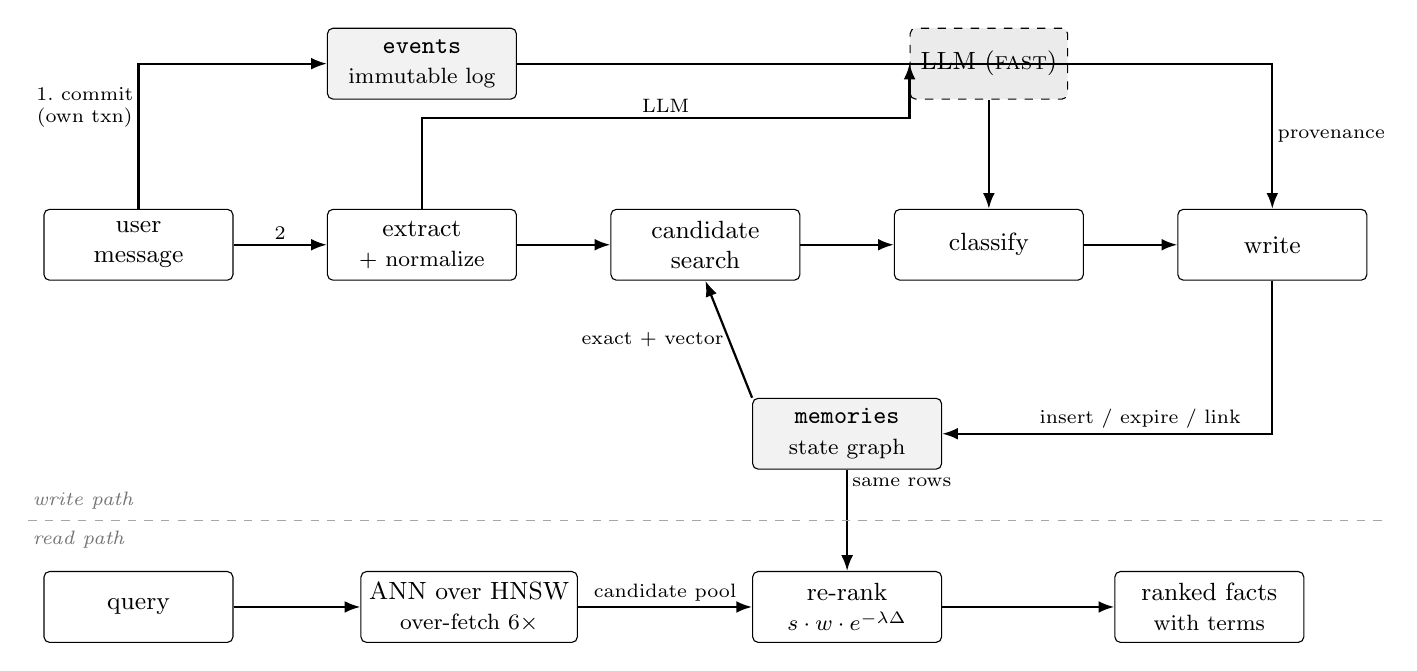
\begin{tikzpicture}[x=1cm, y=1cm,
  box/.style={draw, rounded corners=2pt, align=center, minimum height=9mm,
              minimum width=24mm, inner sep=3pt, font=\small},
  store/.style={box, fill=black!5},
  llm/.style={box, fill=black!8, dashed, minimum width=20mm},
  ar/.style={-{Latex[length=2mm]}, thick},
  lbl/.style={font=\scriptsize, inner sep=1.5pt, align=center}
]
% --- write path (upper) -------------------------------------------------
\node[box]   (msg)  at (0,0)    {user\\message};
\node[box]   (ex)   at (3.6,0)  {extract\\\footnotesize + normalize};
\node[box]   (cand) at (7.2,0)  {candidate\\search};
\node[box]   (cls)  at (10.8,0) {classify};
\node[box]   (wr)   at (14.4,0) {write};
\node[store] (ev)   at (3.6,2.3) {\texttt{events}\\\footnotesize immutable log};
\node[llm]   (llmn) at (10.8,2.3) {LLM (\textsc{fast})};
\node[store] (mem)  at (9.0,-2.4) {\texttt{memories}\\\footnotesize state graph};

\draw[ar] (msg) |- node[lbl, left, pos=0.35] {1.\ commit\\(own txn)} (ev.west);
\draw[ar] (msg) -- node[lbl, above] {2} (ex);
\draw[ar] (ex)   -- (cand);
\draw[ar] (cand) -- (cls);
\draw[ar] (cls)  -- (wr);
\draw[ar] (llmn) -- (cls);
\draw[ar] (ex.north) -- ++(0,1.15) -| node[lbl, above, pos=0.25] {LLM} (llmn.west);
\draw[ar] (ev.east) -| node[lbl, right, pos=0.75] {provenance} (wr.north);
\draw[ar] (mem.north west) -- node[lbl, left] {exact + vector} (cand.south);
\draw[ar] (wr.south) |- node[lbl, above, pos=0.7] {insert / expire / link} (mem.east);

% --- read path (lower) --------------------------------------------------
\node[box] (q)   at (0,-4.6)    {query};
\node[box] (ann) at (4.2,-4.6)  {ANN over HNSW\\\footnotesize over-fetch $6\times$};
\node[box] (rr)  at (9.0,-4.6)  {re-rank\\\footnotesize $s \cdot w \cdot e^{-\lambda\Delta}$};
\node[box] (out) at (13.6,-4.6) {ranked facts\\\footnotesize with terms};

\draw[ar] (q)   -- (ann);
\draw[ar] (ann) -- node[lbl, above] {candidate pool} (rr);
\draw[ar] (rr)  -- (out);
\draw[ar] (mem.south) -- node[lbl, right, pos=0.12] {same rows} (mem.south |- ann.north);

\draw[dashed, black!35] (-1.4,-3.5) -- (15.8,-3.5);
\node[lbl, anchor=west, black!55] at (-1.4,-3.25) {\textit{write path}};
\node[lbl, anchor=west, black!55] at (-1.4,-3.75) {\textit{read path}};
\end{tikzpicture}}
\caption{The DTSG architecture. The upper path is the write pipeline: the raw
message is committed to the immutable event log \emph{first, in its own
transaction}, and only then is derived state computed --- extraction,
two-armed candidate search, LLM classification, and an atomic
insert-and-expire. The lower path is retrieval: Postgres performs approximate
nearest-neighbour search over the HNSW index and deliberately over-fetches,
because top-$K$ by cosine is not top-$K$ by the full score; Python then applies
the temporal re-ranking formula of Equation~\eqref{eq:score}. Dashed nodes are
language-model calls.}
\label{fig:arch}
\end{figure}

\subsubsection{The write pipeline}

The ingest path is
\[
\text{message} \rightarrow \text{event (committed)} \rightarrow \text{facts}
\rightarrow \text{candidates} \rightarrow \text{classification}
\rightarrow \text{writes}.
\]

\paragraph{The event commits first, alone.} Extraction and classification both
call a language model, so both can fail on a rate limit or a timeout. If the
whole flow shared one transaction, such a failure would roll back the raw
message too --- and the raw message is the one thing that cannot be
reconstructed. Memories can always be rebuilt by replaying events; events
cannot be rebuilt from anything. So the log commits in its own transaction and
a downstream failure costs derived state, never history. Each fact is then
applied in its own transaction, so one fact's failure does not undo its
predecessors' writes.

\paragraph{Immutability is enforced, not intended.} Migration 0002 places
\texttt{BEFORE UPDATE} and \texttt{BEFORE DELETE} triggers on \texttt{events}
that reject the operation for every role, service role included. Before this,
``append-only'' was a convention one careless query away from being false.
Genuine deletions do eventually become necessary (an erasure request, a test
teardown), so there is a deliberate, transaction-scoped escape hatch:

\begin{lstlisting}[language=SQL]
begin;
set local dtsg.allow_event_mutation = 'on';
delete from events where user_id = '...';
commit;
\end{lstlisting}

\noindent \texttt{set local} scopes the exemption to the transaction, so it
cannot leak into the pooled connection's next user, and application code never
sets it. Erasing history stays possible, but never accidental.

\paragraph{Candidate search has two arms}, because they fail in opposite
directions. The \textbf{exact} arm matches on \texttt{(user\_id, subject,
predicate)} and is always included regardless of vector distance: if the user
already has a \texttt{lives\_in} fact, a new one must be considered even when
Delhi and Berlin embed far apart. The \textbf{vector} arm retrieves
semantically near facts above a similarity floor of $0.55$, catching overlap the
exact arm misses --- an older \texttt{works\_at} against a new
\texttt{works\_as}, for instance. The union is passed to the classifier.

\paragraph{The classification.} An LLM assigns one of three resolutions:

\begin{center}
\begin{tabular}{ll}
\textsc{reinforce} & the new fact restates a held one; raise its confidence, store no copy\\
\textsc{additive}  & the new fact coexists with everything; store it, touch nothing\\
\textsc{supersede} & the new fact makes held facts untrue; store it, expire and link them\\
\end{tabular}
\end{center}

\noindent The decision that matters is \textsc{additive} vs.\ \textsc{supersede},
and it is \emph{not} ``same subject and predicate'':
\begin{align*}
\texttt{user speaks English} \;+\; \texttt{user speaks Hindi}\;\;   &\rightarrow\;\; \textsc{additive} \quad\text{(multi-valued)}\\
\texttt{user lives\_in Delhi} \;+\; \texttt{user lives\_in Berlin}\;\; &\rightarrow\;\; \textsc{supersede} \quad\text{(single-valued)}
\end{align*}
Both pairs share a subject and a predicate. Treating that as contradiction
would silently delete the user's second language; treating it as coexistence
would leave them living in two cities. Nothing in the schema decides this --- it
is a judgement about whether a predicate can hold several values at once, which
is why a language model makes the call, prompted with explicit single-valued and
multi-valued exemplars.

The error policy is deliberately \textbf{asymmetric}. A wrong \textsc{additive}
leaves a stale fact \texttt{ACTIVE}, which the retrieval ranking moderates and a
later correction repairs. A wrong \textsc{supersede} expires something true; the
row survives, but it drops out of ``what is true now'' until someone notices. So
the prompt instructs the model to choose \textsc{additive} when genuinely
unsure. Two further guards run after the model returns: a \textsc{reinforce} or
\textsc{supersede} naming no known memory is downgraded to \textsc{additive}
(a \textsc{supersede} with no valid target would expire nothing while still
writing a new fact, producing exactly the contradiction the phase exists to
prevent), and a \textsc{reinforce} naming several rows is trimmed to the closest
one, since reinforcing several at once would inflate confidence across facts the
user restated only one of. When the candidate list is empty the model is not
called at all --- no candidates means no possible conflict, which removes any
chance of a hallucinated target on what is also the most common path.

\paragraph{The write.} On \textsc{supersede} the new memory is inserted and the
targets are expired \emph{in the same transaction}: \texttt{status =
'EXPIRED'}, \texttt{valid\_until = now()}, and \texttt{superseded\_by} set to
the new row. Atomicity is required in both directions --- a crash between the
two statements would either leave two contradictory \texttt{ACTIVE} facts or
expire the old fact with nothing replacing it. The expiry is guarded on
\texttt{status = 'ACTIVE'} so a retry cannot overwrite a chain link written by
the first attempt. Algorithm~\ref{alg:ingest} states the pipeline.

\begin{algorithm}[htbp]
\caption{DTSG ingest --- from a message to a consistent state graph}
\label{alg:ingest}
\begin{algorithmic}[1]
\Procedure{Ingest}{$u$: user, $m$: message}
  \State $e \gets$ \Call{InsertEvent}{$u, m$} \Comment{own transaction; commits before anything derived}
  \State $R \gets$ \Call{ExtractFacts}{$m$} \Comment{LLM, schema-enforced triples}
  \State $F \gets$ \Call{Normalize}{$R$} \Comment{subject folding, snake\_case, synonym map}
  \For{each fact $f \in F$}
    \State $v \gets$ \Call{Embed}{$f$} \Comment{null on failure; degrade, do not drop}
    \State $C \gets$ \Call{ExactMatch}{$u, f$} $\cup$ \Call{VectorMatch}{$u, v$} \Comment{similarity floor $0.55$}
    \If{$C = \emptyset$}
      \State $(r, T) \gets (\textsc{additive}, \emptyset)$ \Comment{no candidates, no possible conflict}
    \Else
      \State $(r, T) \gets$ \Call{Classify}{$f, C$} \Comment{LLM; targets reconciled against $C$}
    \EndIf
    \If{$r = \textsc{reinforce}$}
      \State \Call{BumpConfidence}{$T_1$} \Comment{also stamps \texttt{last\_reinforced\_at}}
    \Else
      \State \textbf{begin transaction}
      \State $n \gets$ \Call{InsertMemory}{$u, f, v, e$}
      \If{$r = \textsc{supersede}$}
        \State \Call{Expire}{$T$, $n$} \Comment{sets \texttt{superseded\_by}; guarded on ACTIVE}
      \EndIf
      \State \textbf{commit}
    \EndIf
  \EndFor
\EndProcedure
\end{algorithmic}
\end{algorithm}

\subsubsection{Temporal retrieval}

Retrieval is where the temporal structure is cashed in. Every candidate is
scored as
\begin{equation}
\label{eq:score}
\mathrm{score}(f, q, t) \;=\; \underbrace{\max\!\big(0,\ \cos(\mathbf{e}_f, \mathbf{e}_q)\big)}_{\text{is it relevant}}
\;\times\; \underbrace{w(f, t)}_{\text{is it still true}}
\;\times\; \underbrace{e^{-\lambda\,\Delta(f,t)}}_{\text{how stale is it}},
\end{equation}
where $\mathbf{e}_f$ and $\mathbf{e}_q$ are the fact and query embeddings,
$t$ is the reference time of the query, $\Delta(f,t)$ is the age in days, and
the status weight is evaluated \emph{against $t$} rather than read from the
stored column:
\begin{equation}
\label{eq:weight}
w(f,t) \;=\;
\begin{cases}
w_{\text{exp}}, & \text{if } \texttt{valid\_from}(f) > t \quad \text{(it had not happened yet)}\\[2pt]
1.0, & \text{if } \texttt{valid\_until}(f) = \textsc{null} \ \text{ or } \ \texttt{valid\_until}(f) > t\\[2pt]
w_{\text{exp}}, & \text{otherwise (it had already stopped being true)}
\end{cases}
\end{equation}
with $w_{\text{exp}} = 0.15$ by default. The age is measured from a reference
instant that differs by status: for an \texttt{ACTIVE} fact it is
\texttt{last\_reinforced\_at} if the fact has been restated, else
\texttt{valid\_from}; for an \texttt{EXPIRED} fact it is \texttt{valid\_until},
so that among superseded facts the recently changed ones rank highest --- which
is what makes ``what changed lately'' answerable by the same formula. The delta
is clamped at zero, so a fact timestamped slightly ahead of $t$ (clock skew, or
an \texttt{as\_of} between \texttt{valid\_from} and now) cannot produce a
negative exponent and outrank everything. Cosine similarity is clamped at zero
for the same class of reason: it runs $[-1,1]$, and a negative value would flip
the sign of the whole product and turn an irrelevant fact into a top hit.

The decay constant defaults to $\lambda = \ln(2)/180$, a 180-day half-life.
Facts people state about themselves age slowly --- a city or a job stays true
for months or years --- so more aggressive decay buries correct answers faster
than they actually go stale. Both $\lambda$ and $w_{\text{exp}}$ are
per-request parameters, so a test set can be swept without a redeployment;
Section~\ref{sec:results} uses exactly this to ablate the terms.

\paragraph{Three modes, one store.} Equation~\eqref{eq:weight} is what turns
different temporal questions into one query with a different $t$:

\begin{center}
\begin{tabular}{lll}
\toprule
\textbf{Mode} & \textbf{Eligible rows} & \textbf{Scored at}\\
\midrule
\texttt{now} (default) & everything; superseded rows discounted & now\\
\texttt{as\_of} & only facts that held at that instant & the given \texttt{as\_of}\\
\texttt{changes} & only rows in a supersede chain, newest transition first & now\\
\bottomrule
\end{tabular}
\end{center}

\noindent Because \texttt{as\_of} evaluates the status term against that moment,
a fact superseded last week counts as fully current for a question about last
month. ``What did I say before X'' therefore becomes a ranking question rather
than a separate store.

\paragraph{Two-stage re-ranking.} No index can be built over
Equation~\eqref{eq:score}, because its terms depend on query time and on
caller-supplied constants. So Postgres does the part it is good at ---
approximate nearest-neighbour search over the HNSW cosine index --- and Python
applies the full score to the returned pool. The pool is deliberately
over-fetched at $6\times$ the requested limit with a floor of 40, because
top-$K$ by cosine is \emph{not} top-$K$ by score: a fact that wins on the full
formula can sit outside the cosine top-$K$ and would be silently dropped by a
tight pool. Each response reports \texttt{candidates\_considered} so a caller
can tell whether the pool saturated, and returns the three terms of
Equation~\eqref{eq:score} separately rather than only their product --- a
ranking that cannot be decomposed is a ranking that cannot be debugged.

\subsubsection{The timeline view}

\texttt{GET /api/timeline} walks the supersede links into chains, oldest first,
and the frontend renders them with current values marked and superseded ones
struck through with their validity range (Figure~\ref{fig:chain}). The walk
follows \texttt{superseded\_by} rather than \texttt{supersedes}, because that is
the complete edge: when one fact invalidates several, each old row records the
replacement, while the new row's single \texttt{supersedes} column can only name
one of them. A fact that was never superseded comes back as a chain of one, so
the UI needs a single rendering path rather than separate ``history'' and ``just
a fact'' cases. Dangling links (a replacement outside the current page) stop the
walk instead of inventing entries, and cycles --- which the write path should
make impossible --- surface their rows rather than hanging or silently dropping
them.

\begin{figure}[htbp]
\centering
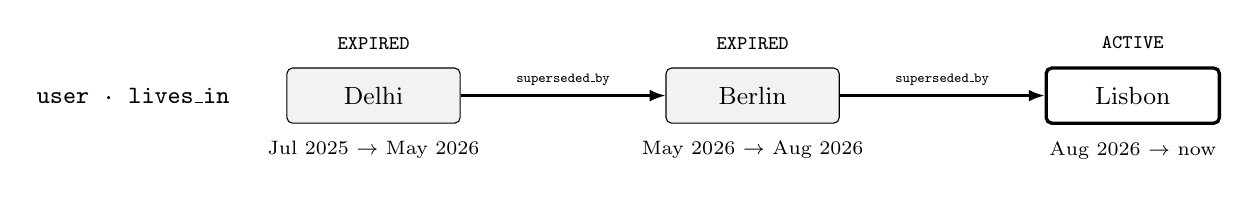
\begin{tikzpicture}[
  n/.style={draw, rounded corners=2pt, minimum width=22mm, minimum height=7mm, font=\small},
  old/.style={n, fill=black!5},
  cur/.style={n, very thick},
  ar/.style={-{Latex[length=2mm]}, thick}
]
\node[old] (a) {Delhi};
\node[old, right=26mm of a] (b) {Berlin};
\node[cur, right=26mm of b] (c) {Lisbon};
\node[font=\scriptsize, below=1mm of a] {Jul 2025 $\to$ May 2026};
\node[font=\scriptsize, below=1mm of b] {May 2026 $\to$ Aug 2026};
\node[font=\scriptsize, below=1mm of c] {Aug 2026 $\to$ now};
\node[font=\scriptsize, above=1mm of a] {\texttt{EXPIRED}};
\node[font=\scriptsize, above=1mm of b] {\texttt{EXPIRED}};
\node[font=\scriptsize, above=1mm of c] {\texttt{ACTIVE}};
\draw[ar] (a) -- node[above,font=\tiny]{\texttt{superseded\_by}} (b);
\draw[ar] (b) -- node[above,font=\tiny]{\texttt{superseded\_by}} (c);
\node[left=6mm of a, font=\small] {\texttt{user · lives\_in}};
\end{tikzpicture}
\caption{A supersede chain as rendered by the timeline view. No row is ever
deleted: two moves produce three rows, of which one is \texttt{ACTIVE} and two
are \texttt{EXPIRED} with closed validity intervals. The chain is walked along
\texttt{superseded\_by}, which is the authoritative edge because a single fact
may invalidate several predecessors.}
\label{fig:chain}
\end{figure}

% ================================================================
\section{Experiment Design}
\label{sec:exp}

Three experiments were run, each isolating a different variable.

\paragraph{E1 --- Policy comparison (DTSG vs.\ naive RAG).} The question is
whether temporal ranking beats similarity ranking on the cases where the two can
disagree. The two policies are:
\begin{itemize}
  \item \textbf{Baseline (naive RAG):} rank by cosine similarity alone, ties
        broken by input order, exactly as a database returning rows in index
        order would. No status weighting, no decay, no re-ranking.
  \item \textbf{DTSG:} rank by Equation~\eqref{eq:score} with default
        parameters $w_{\text{exp}} = 0.15$, $\lambda = \ln(2)/180$.
\end{itemize}
Input is the 4-case set of Table~\ref{tab:cases}; output is the top-ranked fact
per case under each policy. Two metrics are recorded: \emph{correct top hit},
counted over the 3 scored cases, and \emph{stale top hit} (the top-ranked fact
has status \texttt{EXPIRED}), counted over all 4. The second metric matters
independently, because a system can be accidentally right about which object to
return while still promoting a fact it should know is dead.

\textbf{The critical design choice is that the cases carry their own similarity
scores}, so no embedding model runs. Using real embeddings would make the result
depend on the embedding model's quality, which is not the thing under test; by
fixing similarity, any difference in outcome is attributable to the ranking
policy alone.

\paragraph{On the fairness of the comparison.} Both policies read the same
\texttt{memories} rows, which might look like DTSG is being handed a curated
corpus. It is not, and the equivalence is worth stating precisely: a naive store
never expires anything, so its corpus is ``every fact ever extracted'' --- and
DTSG never deletes anything either, it only marks rows \texttt{EXPIRED}. The row
sets are identical. The baseline simply ignores the status and time columns,
exactly as a system that never wrote them would, which isolates the retrieval
policy as the only variable. One caveat runs in the other direction:
DTSG's \textsc{reinforce} collapses a restatement into a confidence bump rather
than a second row, so a truly naive store would hold a few more near-duplicates
than this baseline sees. Duplicates make naive retrieval look more consistent,
so the measurement is conservative rather than flattering. The same comparison
is available on live data through \texttt{POST /api/baseline/compare}, which
runs both policies on one query and reports where they diverge.

\paragraph{E2 --- Term ablation on a controlled scenario.} The question is which
term of Equation~\eqref{eq:score} does the work. A scenario is constructed in
which the user moved from Delhi to Berlin 10 days ago and \emph{both facts have
cosine similarity exactly 1.000}, so the similarity term is held constant by
construction and a vector store cannot distinguish them even in principle. Four
configurations are run over the same two rows:
(i) \texttt{mode=now} with defaults;
(ii) $w_{\text{exp}} = 1.0$, which removes the status penalty;
(iii) \texttt{mode=as\_of} 60 days ago, which moves the reference time to before
the move;
(iv) $\lambda = 0$, which removes decay and isolates the status term.
Output for each is the score of both facts with the three terms reported
separately.

\paragraph{E3 --- Correctness of the pipeline.} The question is whether the
write path maintains the invariants the design depends on. A suite of 103
automated tests covers extraction and normalization, the classifier's coercion
guards, event immutability and keyset pagination, the insert-and-expire
transaction, chain walking including dangling links and cycles, retrieval
scoring and re-ranking, and the baseline endpoints. The language-model provider
is stubbed throughout, so the suite tests the system rather than the model, and
runs without a database or an API key.

\paragraph{Setup.} Backend: Python 3, FastAPI, asyncpg, deployed on Render;
database: Supabase Postgres with \texttt{pgvector}, \texttt{vector(1536)} and an
HNSW cosine index; models: \texttt{gemini-2.5-flash} for extraction and
classification, \texttt{gemini-embedding-001} at 1536 dimensions for embeddings;
frontend: React + TypeScript + Vite on Vercel. E1, E2 and E3 all run offline
(\texttt{scripts/run\_benchmark.py}, \texttt{scripts/check\_retrieval.py} and
\texttt{pytest} respectively).

% ================================================================
\section{Results \& Observations}
\label{sec:results}

\paragraph{E1 --- DTSG vs.\ naive RAG.} Table~\ref{tab:e1} gives the per-case
outcome and Table~\ref{tab:e1sum} the aggregate. The separation is complete on
this set: the baseline returns a stale fact as its top hit in 3 of 4 cases and
gets 0 of 3 scored cases right, while DTSG gets 3 of 3 right and never tops a
stale fact.

\begin{table}[htbp]
\centering
\caption{E1 --- top-ranked fact per case under each policy. The baseline is
wrong in every scored case; note that it is wrong for a different reason each
time --- once because the stale fact is more similar, once because the two are
exactly tied, once because the stale fact is much more similar.}
\label{tab:e1}
\small
\begin{tabularx}{\textwidth}{X l l c}
\toprule
\textbf{Query} & \textbf{Baseline top hit} & \textbf{DTSG top hit} & \textbf{DTSG correct?}\\
\midrule
where do I live? & Delhi (\texttt{EXPIRED}) & Berlin (\texttt{ACTIVE}) & yes\\
where do I work? & Acme (\texttt{EXPIRED}) & Globex (\texttt{ACTIVE}) & yes\\
what is my job title? & Engineer (\texttt{EXPIRED}) & Staff Engineer (\texttt{ACTIVE}) & yes\\
which languages do I speak? (control) & English (\texttt{ACTIVE}) & Hindi (\texttt{ACTIVE}) & n/a (either valid)\\
\bottomrule
\end{tabularx}
\end{table}

\begin{table}[htbp]
\centering
\caption{E1 --- aggregate. ``Correct top hit'' is counted over the 3 scored
cases; ``stale top hit'' over all 4.}
\label{tab:e1sum}
\begin{tabular}{lcc}
\toprule
\textbf{Metric} & \textbf{DTSG} & \textbf{Naive RAG baseline}\\
\midrule
Correct top hit $\uparrow$ & \textbf{3/3} & 0/3\\
Stale top hit $\downarrow$ & \textbf{0/4} & 3/4\\
\bottomrule
\end{tabular}
\end{table}

The control case is the informative one for the opposite failure mode. ``Which
languages do I speak?'' has two \texttt{ACTIVE} facts, English and Hindi, with
identical similarity; DTSG returns Hindi on top purely because it is more
recent, and English remains in the result set. Had the classifier been
over-eager and treated \texttt{speaks} as single-valued, one of the two would
have been expired at write time and this case would have looked like a success
in the aggregate while having silently destroyed a true fact. The case is in the
set specifically to make that failure visible, and it does not occur.

\paragraph{E2 --- which term does the work.} Table~\ref{tab:e2} reports the
controlled Delhi/Berlin scenario. Because similarity is pinned at 1.000 for both
rows, every difference in the table is produced by the status and recency terms.

\begin{table}[htbp]
\centering
\caption{E2 --- term ablation on the Delhi $\to$ Berlin scenario (moved 10 days
ago). Both facts have cosine similarity 1.000 by construction, so a cosine-only
ranker sees one number for both rows and cannot choose. Bold marks the top hit.}
\label{tab:e2}
\small
\begin{tabular}{llccccl}
\toprule
\textbf{Configuration} & \textbf{Fact} & \textbf{sim.} & \textbf{status $w$} & \textbf{recency} & \textbf{score} & \\
\midrule
\texttt{mode=now} (defaults) & Berlin & 1.000 & 1.00 & 0.962 & \textbf{0.9622} & \\
                             & Delhi  & 1.000 & 0.15 & 0.962 & 0.1443 & \\
\addlinespace
$w_{\text{exp}}=1.0$ (``where have I lived?'') & Berlin & 1.000 & 1.00 & 0.962 & 0.9622 & \\
                             & Delhi  & 1.000 & 1.00 & 0.962 & 0.9622 & \\
\addlinespace
\texttt{mode=as\_of}, $-60$ days & Delhi  & 1.000 & 1.00 & 1.000 & \textbf{1.0000} & \\
                             & Berlin & 1.000 & 0.15 & 1.000 & 0.1500 & \\
\addlinespace
$\lambda = 0$ (no decay) & Berlin & 1.000 & 1.00 & 1.000 & \textbf{1.0000} & \\
                             & Delhi  & 1.000 & 0.15 & 1.000 & 0.1500 & \\
\bottomrule
\end{tabular}
\end{table}

Three observations follow. First, \textbf{the status term is doing the work}:
with decay switched off entirely ($\lambda = 0$), the separation is still
$1.0000$ vs.\ $0.1500$ --- a factor of $1/w_{\text{exp}}$ --- whereas the
recency term contributes only the common factor $0.962$ over a 10-day gap. Decay
matters for ordering several live facts (as in the control case of E1), not for
separating live from dead. Second, \textbf{the discount is a discount, not a
filter}: raising $w_{\text{exp}}$ to 1.0 brings Delhi back to parity in the same
query against the same store, which is what makes ``where have I lived?''
answerable without a second index. Third, \textbf{the ordering inverts under
\texttt{as\_of}}: asked about a date 60 days ago, Delhi scores 1.0000 and Berlin
0.1500, because Equation~\eqref{eq:weight} is evaluated at the query's reference
time and at that instant Berlin had not happened yet. That inversion is not
special-cased anywhere; it falls out of the formula.

\paragraph{E3 --- pipeline correctness.} All 103 tests pass
(\texttt{103 passed in 1.21s}), covering extraction and normalization, the
classifier's target-reconciliation guards, event immutability and keyset
pagination, the atomic insert-and-expire, chain walking with dangling links and
cycles, the scoring and re-ranking functions, and the baseline endpoints.

\paragraph{What works, and why.} The gain in E1 is not an artefact of tuning; it
is structural. Cosine similarity measures whether two strings are \emph{about}
the same thing, and ``I live in Delhi'' and ``I live in Berlin'' are maximally
about the same thing --- which is exactly why similarity cannot separate them.
Any amount of embedding-model improvement makes this worse rather than better,
since a better model brings the two closer together. The information needed to
choose is not in the text at all; it is in the write-time record of which one
replaced the other. DTSG wins these cases because it \emph{stored that record},
and the retrieval formula is only the place where the stored record is spent.

\paragraph{What does not work, and why.} Four limitations are visible in these
results and should temper them.

\begin{enumerate}
  \item \textbf{The benchmark is small and adversarial by construction.} Four
        cases, hand-written, all chosen so that similarity alone fails. A 3/3
        vs.\ 0/3 result on such a set demonstrates that the mechanism operates
        as designed; it does not estimate an accuracy on a realistic query
        distribution, where most questions have no competing stale fact and both
        policies would agree. The honest reading is that DTSG is never worse
        here and is decisively better on the subset that matters, not that it is
        ``100\% accurate''.
  \item \textbf{The upstream stages are not evaluated against a live model.}
        E1 and E2 hold similarity fixed and E3 stubs the provider, so extraction
        quality and the classifier's single- vs.\ multi-valued judgement are
        unproven end to end. Everything downstream ranks whatever those two
        stages write: a missed \textsc{supersede} leaves two \texttt{ACTIVE}
        facts and the ranking will faithfully return the wrong one.
        \texttt{scripts/check\_extraction.py} and
        \texttt{scripts/check\_classifier.py} exist to run these against a real
        key, and doing so is the first item of future work.
  \item \textbf{The parameters are chosen, not learned.} $w_{\text{exp}} = 0.15$
        and a 180-day half-life are defensible defaults --- the first is low
        enough that a stale fact never outranks a live one on similar text and
        high enough to stay reachable, the second reflects that self-reported
        facts age slowly --- but neither is fitted to data. They are per-request
        parameters precisely so that they can be swept once a labelled set
        exists.
  \item \textbf{Normalization is a finite table.} 15 canonical predicates and 22
        synonyms cover the common cases, but a predicate the table does not know
        will not match its own earlier variant, and the resulting failure is
        silent: no conflict is detected, so no supersede occurs, and the graph
        accumulates contradictory \texttt{ACTIVE} facts that retrieval will
        rank in good faith.
\end{enumerate}

% ================================================================
\section{Future Work and Conclusion}
\label{sec:conclusion}

\paragraph{Who benefits.} Any system that must remember a person across
sessions and get the \emph{current} answer right: conversational assistants,
customer-support agents holding an account's history, tutoring systems tracking
what a learner has mastered, and health or finance applications where an
out-of-date fact is not merely unhelpful but harmful. The immutable log with a
scoped erasure hatch is also directly useful for auditability and for handling
erasure requests without abandoning append-only semantics elsewhere.

\paragraph{Limitations.} Beyond the four listed in Section~\ref{sec:results}:
the classifier makes one language-model call per extracted fact against its
candidate set, so ingest cost grows with the number of facts per message rather
than with messages; the state graph is flat subject--predicate--object, with no
entity resolution, so ``Acme'' and ``Acme Corp.'' remain distinct objects; the
\texttt{supersedes} column holds a single uuid, so when one fact invalidates
several the complete edge set lives only on the \texttt{superseded\_by} side;
and there is no consolidation or summarization step, so a very long-lived user
accumulates rows indefinitely.

\paragraph{Future work.} In rough order of value:
(1) \textbf{run the live-model checks} and measure extraction precision/recall
and classifier agreement against a hand-labelled set --- this is the largest
open gap;
(2) \textbf{evaluate on a public benchmark}, specifically the knowledge-update
subsets of LongMemEval~\cite{wu2024longmemeval} and
LoCoMo~\cite{maharana2024locomo}, which would place these results on the same
axis as Zep and Mem0;
(3) \textbf{sweep $w_{\text{exp}}$ and $\lambda$} on that labelled set, and
consider learning a per-predicate half-life, since a job title and a mood do not
age at the same rate;
(4) \textbf{learn the single-/multi-valued property per predicate} from
observed supersede history instead of asking the model each time, which would
cut both cost and variance on the decision that matters most;
(5) \textbf{entity resolution} over objects, so surface variants of one employer
or city collapse;
(6) \textbf{answer generation}, wiring the \textsc{smart} tier (currently
reserved and called by no endpoint) to produce answers grounded in the retrieved,
status-annotated facts, with citations to \texttt{source\_event};
(7) \textbf{multi-hop retrieval} over the graph, as in
HippoRAG~\cite{gutierrez2024hipporag}, which the current single-hop scoring does
not attempt.

\paragraph{Conclusion.} We set out to fix a specific and quiet failure: agent
memory that answers with a fact that used to be true. The diagnosis is that
similarity search has no way to represent the relation between an old fact and
the one that replaced it, so the information needed to choose correctly is
absent at read time --- which is a write-time problem wearing a read-time
disguise. DTSG's response is to record that relation when the contradiction
occurs: an immutable event log preserves what was said, a mutable state graph
records what is currently believed, and a supersede link joins the two states of
every changed fact instead of deleting either. Retrieval then spends that record
through one decomposable product of relevance, validity and staleness, whose
status term is evaluated at the query's reference time --- so ``where do I
live?'' and ``where did I live in the spring?'' are the same query with a
different parameter, and both are answered from one store. On a benchmark built
from exactly the cases where similarity cannot help, this moves the correct top
hit from 0/3 to 3/3 and eliminates stale top hits entirely, with a term ablation
showing that the status weight rather than recency decay is what produces the
separation. The measured gains come from a small adversarial set and the
upstream extraction and classification stages remain unvalidated against a live
model, so the result should be read as evidence that the mechanism works as
designed rather than as an accuracy claim; closing that gap is the immediate
next step.

% ================================================================
\clearpage
\begin{thebibliography}{99}\small

\bibitem{rasmussen2025zep}
Preston Rasmussen, Pavlo Paliychuk, Travis Beauvais, Jack Ryan, and Daniel Chalef.
Zep: A temporal knowledge graph architecture for agent memory.
\textit{arXiv preprint arXiv:2501.13956}, 2025.

\bibitem{chhikara2025mem0}
Prateek Chhikara, Dev Khant, Saket Aryan, Taranjeet Singh, and Deshraj Yadav.
Mem0: Building production-ready AI agents with scalable long-term memory.
\textit{arXiv preprint arXiv:2504.19413}, 2025.

\bibitem{packer2023memgpt}
Charles Packer, Sarah Wooders, Kevin Lin, Vivian Fang, Shishir G. Patil, Ion Stoica, and Joseph E. Gonzalez.
MemGPT: Towards LLMs as operating systems.
\textit{arXiv preprint arXiv:2310.08560}, 2023.

\bibitem{park2023generativeagents}
Joon Sung Park, Joseph C. O'Brien, Carrie J. Cai, Meredith Ringel Morris, Percy Liang, and Michael S. Bernstein.
Generative agents: Interactive simulacra of human behavior.
In \textit{Proceedings of the 36th Annual ACM Symposium on User Interface Software and Technology (UIST)}, 2023.

\bibitem{zhong2023memorybank}
Wanjun Zhong, Lianghong Guo, Qiqi Gao, He Ye, and Yanlin Wang.
MemoryBank: Enhancing large language models with long-term memory.
\textit{arXiv preprint arXiv:2305.10250}, 2023.

\bibitem{xu2025amem}
Wujiang Xu, Zujie Liang, Kai Mei, Hang Gao, Juntao Tan, and Yongfeng Zhang.
A-MEM: Agentic memory for LLM agents.
\textit{arXiv preprint arXiv:2502.12110}, 2025.

\bibitem{wu2024longmemeval}
Di Wu, Hongwei Wang, Wenhao Yu, Yuwei Zhang, Kai-Wei Chang, and Dong Yu.
LongMemEval: Benchmarking chat assistants on long-term interactive memory.
\textit{arXiv preprint arXiv:2410.10813}, 2024.

\bibitem{maharana2024locomo}
Adyasha Maharana, Dong-Ho Lee, Sergey Tulyakov, Mohit Bansal, Francesco Barbieri, and Yuwei Fang.
Evaluating very long-term conversational memory of LLM agents.
In \textit{Proceedings of the 62nd Annual Meeting of the Association for Computational Linguistics (ACL)}, 2024.

\bibitem{gutierrez2024hipporag}
Bernal Jim\'enez Guti\'errez, Yiheng Shu, Yu Gu, Michihiro Yasunaga, and Yu Su.
HippoRAG: Neurobiologically inspired long-term memory for large language models.
In \textit{Advances in Neural Information Processing Systems (NeurIPS)}, 2024.

\bibitem{lewis2020rag}
Patrick Lewis, Ethan Perez, Aleksandra Piktus, Fabio Petroni, Vladimir Karpukhin, Naman Goyal, et al.
Retrieval-augmented generation for knowledge-intensive NLP tasks.
In \textit{Advances in Neural Information Processing Systems (NeurIPS)}, 2020.

\bibitem{asai2024selfrag}
Akari Asai, Zeqiu Wu, Yizhong Wang, Avirup Sil, and Hannaneh Hajishirzi.
Self-RAG: Learning to retrieve, generate, and critique through self-reflection.
In \textit{International Conference on Learning Representations (ICLR)}, 2024.

\bibitem{vu2023freshllms}
Tu Vu, Mohit Iyyer, Xuezhi Wang, Noah Constant, Jerry Wei, Jason Wei, et al.
FreshLLMs: Refreshing large language models with search engine augmentation.
\textit{arXiv preprint arXiv:2310.03214}, 2023.

\bibitem{dhingra2022templama}
Bhuwan Dhingra, Jeremy R. Cole, Julian Martin Eisenschlos, Daniel Gillick, Jacob Eisenstein, and William W. Cohen.
Time-aware language models as temporal knowledge bases.
\textit{Transactions of the Association for Computational Linguistics}, 10:257--273, 2022.

\bibitem{chen2021timeqa}
Wenhu Chen, Xinyi Wang, and William Yang Wang.
A dataset for answering time-sensitive questions.
In \textit{NeurIPS Datasets and Benchmarks Track}, 2021.

\bibitem{liska2022streamingqa}
Adam Li\v{s}ka, Tom\'a\v{s} Ko\v{c}isk\'y, Elena Gribovskaya, Tayfun Terzi, Eren Sezener, Devang Agrawal, et al.
StreamingQA: A benchmark for adaptation to new knowledge over time in question answering models.
In \textit{International Conference on Machine Learning (ICML)}, 2022.

\bibitem{trivedi2017knowevolve}
Rakshit Trivedi, Hanjun Dai, Yichen Wang, and Le Song.
Know-Evolve: Deep temporal reasoning for dynamic knowledge graphs.
In \textit{International Conference on Machine Learning (ICML)}, 2017.

\bibitem{garciaduran2018learning}
Alberto Garc\'ia-Dur\'an, Sebastijan Duman\v{c}i\'c, and Mathias Niepert.
Learning sequence encoders for temporal knowledge graph completion.
In \textit{Proceedings of EMNLP}, 2018.

\bibitem{jin2020renet}
Woojeong Jin, Meng Qu, Xisen Jin, and Xiang Ren.
Recurrent event network: Autoregressive structure inference over temporal knowledge graphs.
In \textit{Proceedings of EMNLP}, 2020.

\bibitem{cai2023tkgsurvey}
Borui Cai, Yong Xiang, Longxiang Gao, He Zhang, Yunfeng Li, and Jianxin Li.
Temporal knowledge graph completion: A survey.
\textit{arXiv preprint arXiv:2201.08236}, 2023.

\bibitem{meng2022rome}
Kevin Meng, David Bau, Alex Andonian, and Yonatan Belinkov.
Locating and editing factual associations in GPT.
In \textit{Advances in Neural Information Processing Systems (NeurIPS)}, 2022.

\bibitem{meng2023memit}
Kevin Meng, Arnab Sen Sharma, Alex Andonian, Yonatan Belinkov, and David Bau.
Mass-editing memory in a transformer.
In \textit{International Conference on Learning Representations (ICLR)}, 2023.

\bibitem{snodgrass1999developing}
Richard T. Snodgrass.
\textit{Developing Time-Oriented Database Applications in SQL}.
Morgan Kaufmann, 1999.

\end{thebibliography}

\end{document}
